\chapter{Extensão para o \emph{Mozilla Firefox}}
Este capítulo trata da aplicação do algoritmo de agrupamento por nuvens dinâmicas para o refinamento de buscas por imagens na \emph{INTERNET} usando o motor de busca do \emph{Google}. O serviço do \emph{Google} de pesquisa oferece por si uma organização dos resultados em grupos. A diferença da organização do \emph{Google} para a organização proposta é que enquanto os resultados e a busca têm como parâmetro de diferenciação o texto associado aos componentes de busca, este trabalho propõe que a disposição dos resultados seja feita com base no conteúdo das imagens. O fluxo de passos executados pela extensão é representado na Figura \ref{fluxo_aplicacoes}.

% Define block styles
\tikzstyle{decision} = [diamond, draw, fill=blue!20, 
    text width=4.5em, text badly centered, node distance=3cm, inner sep=0pt]
\tikzstyle{block} = [rectangle, draw, fill=blue!20, 
    text width=5em, text centered, rounded corners, minimum height=4em]
\tikzstyle{line} = [draw, -latex']
\tikzstyle{cloud} = [draw, ellipse,fill=red!20, node distance=3cm,
    minimum height=2em]
    
\begin{figure}[htb]
\caption{\label{fluxo_aplicacoes}Fluxograma de execução da aplicação.}
\begin{center}
\begin{tikzpicture}[node distance = 2cm, auto]
    % Place nodes
    \node [block] (init) {Início};
    \node [block, below of=init] (identify) {Carrega Imagens};
    \node [block, right of=identify, node distance=3cm] (descritores) {Gera descritores};
    \node [block, right of=descritores, node distance=3cm] (dynamicClustering) {Agrupamento};
    \node [block, right of=dynamicClustering, node distance=3cm] (resultados) {Exibe Resultados};
    \node [block, above of=resultados] (fim) {Fim};
    % Draw edges
    \path [line] (init) -- (identify);
    \path [line] (identify) -- (descritores);
    \path [line] (descritores) -- (dynamicClustering);
    \path [line] (dynamicClustering) -- (resultados);
    \path [line] (resultados) -- (fim);
    
\end{tikzpicture}
\end{center}
\legend{\textbf{Fonte:} Autoria Própria.}
\end{figure}

\begin{comment}
\begin{figure}[htb]
\caption{\label{fluxo_aplicacoes}Fluxograma de Execução das Aplicações.}
\begin{center}
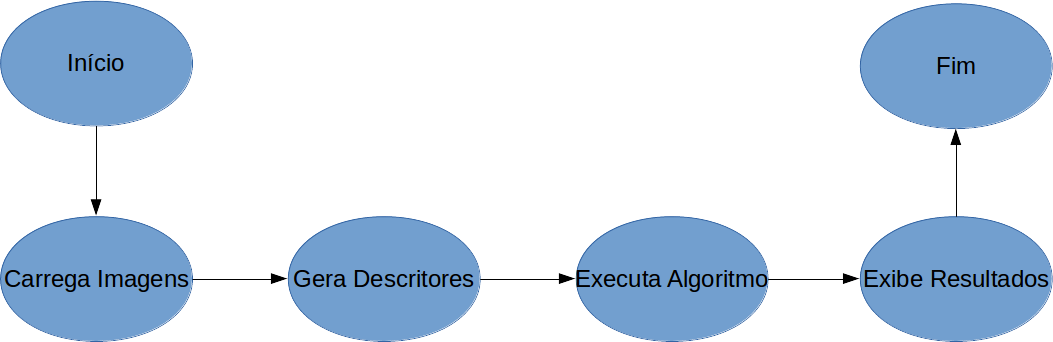
\includegraphics[width=450px]{images/fluxo1.png}
\end{center}
\legend{\textbf{Fonte:} Autoria Própria.}
\end{figure}
\end{comment}

\section{Aplicação}
A extensão do \emph{Mozilla Firefox} foi desenvolvida em \emph{JavaScript} e não altera o modo com que o usuário navega na \emph{INTERNET}, então para que a execução do código seja iniciada é necessário que o usuário acesse a página de resultados de pesquisas de imagens do \emph{Google}. O \emph{Mozilla Firefox} foi escolhido por se tratar de um navegador de código aberto desenvolvido sem fins lucrativos, além disso, o \emph{Mozilla Firefox} é adotado como navegador padrão na maioria dos sistemas operacionais de código aberto e de licença livre.

O Algoritmo \ref{algo_base} é um esboço do que é feito pela aplicação proposta. A extensão verifica a página que está sendo acessada a cada página carregada no navegador, quando a página em questão é a página específica, a extensão exibe uma caixa de diálogo \emph{JavaScript} para que o usuário informe o número de \emph{clusters} desejados como mostra a Figura \ref{input}. De maneira semelhante, o usuário escolhe o descritor a ser usado pelo algoritmo. Isto feito, as imagens são carregadas, os descritores são gerados, o algoritmo executado e o resultado apresentado na própria página.

As imagens que são mostradas como resultado de uma busca por imagens na página do \emph{Google} são os parâmetros de entrada do código. Assim como a maioria dos \emph{Websites} na \emph{INTERNET} as páginas de resultados de buscas do \emph{Google} são compostas por componentes HTML, CSS e códigos \emph{JavaScript}. 

\begin{algorithm}[htb]
\caption{Aplicação do algoritmo de agrupamento por nuvens dinâmicas em imagens da página de resultados do \emph{Google}.}
\label{algo_base}
	\begin{algorithmic}[1]
		\Function{agruparImagens}{\emph{document}}
			\If{\Call{isResultPage}{\emph{document}}}
				\State $imagens \gets document.getElementsByClassName("rg\_ic rg\_i")$
				\State $descritores \gets \Call{GerarDescritores}{\emph{imagens}}$
				\State $clusters \gets \Call{dynamicClustering}{\emph{descritores}}$
				\State $\Call{showResults}{\emph{clusters}}$
			\EndIf
		\EndFunction
	\end{algorithmic}
\end{algorithm}

\begin{figure}[htb]
\begin{center}
  %\caption{Imagem colorida ampliada.}
  %\begin{subfigure}[b]{0.6\textwidth}
  \centering
  \caption{Caixa de diálogo para entrada do número de grupos desejado.}
      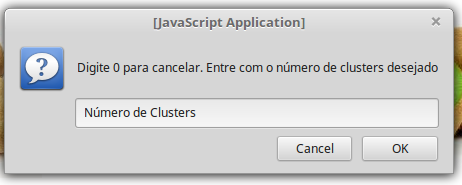
\includegraphics[scale=0.6]{images/input.png}
    
    \label{input}
  %\end{subfigure}
  
  \legend{\textbf{Fonte:} Autoria Própria.}
\end{center}

\end{figure}

A obtenção das imagens da página de resultados do \emph{Google} é possível através de \emph{scripts} \emph{JavaScript} que são capazes de acessar os elementos HTML e suas propriedades. Como descrito anteriormente, os códigos HTML são organizados por componentes e divisores e estes são úteis para exibir o conteúdo da página de maneira estilizada para cada componente e divisão.

O Código \ref{exemplo_simplificado} é um exemplo simplificado de um componente que referencia uma imagem retornada de uma busca. A linha dois do código define o componente que contém a URL da imagem, mas é só na linha três que o componente, que de fato exibe a imagem, é descrito. A imagem referenciada por este componente é representada por uma codificação base 64 e este código está na propriedade \emph{src} do componente da imagem.  
\lstinputlisting[caption={Exemplo Simplificado de Componente \emph{HTML}}, label={exemplo_simplificado},language=HTML]{code/htmlImageExample.html}

Se habilitado no \emph{browser} pelo usuário, os códigos \emph{JavaScript} das páginas na \emph{Web} serão executados. Estes códigos podem estar contidos na própria página a partir dos desenvolvedores da página ou podem ser inseridos de acordo com que as páginas são carregadas no navegador, isto acontece através da ação do próprio navegador ao suportar as extensões.

Sempre que uma página é completamente carregada, um evento é disparado e pode ser identificado por aplicações \emph{JavaScript}. Quando isto acontece, a aplicação desenvolvida neste trabalho varre os elementos HTML em busca de componentes que são da classe \emph{rg\_ic rg\_i}. Esta classe identifica as imagens que são retornadas da busca como mostra o Código \ref{exemplo_simplificado}. A extensão identifica que a página atual contém resultados de busca através do Algoritmo \ref{verifica_pagina}.
\begin{algorithm}[htb]
\caption{Função que verifica se página em questão é página de resultados da busca por imagens.}
\label{verifica_pagina}
	\begin{algorithmic}[1]
	\Function{isResultPage}{\emph{document}}
		\State $imagens \gets document.getElementsByClassName(``rg\_ic\ rg\_i")$
		\State $imagesLength \gets imagens.length$
		\If{$imagensLength > 0$}
			\State \Return $true$
		\Else
			\State \Return $false$
		\EndIf
	\EndFunction
	\end{algorithmic}
\end{algorithm}

Uma vez que as imagens, que serão a entrada do algoritmo são identificadas na página, o algoritmo segue para a fase de geração dos descritores. Nesta fase, a geração do descritor acontece através de um código em \emph{JavaScript} que interage com o componente HTML \emph{canvas} que permite o acesso aos \emph{pixels} das imagens. 

A aplicação suporta o uso dos dois descritores apresentados. A razão para utilização de dois descritores diferentes é que estes são usados pelo algoritmo de agrupamento e dependendo da escolha do descritor, o algoritmo pode apresentar melhor ou pior qualidade em seus resultados.

\begin{comment}
Duas versões da aplicação foram desenvolvidas, as duas versões variam quanto ao uso do descritor. Uma versão utiliza os histogramas das imagens como descritores e outra versão utiliza o autovetor dominante da imagem como descritor. A razão para utilização de dois descritores diferentes é que estes são usados por o algoritmo de agrupamento e dependendo da escolha do descritor, o algoritmo pode apresentar melhor ou pior qualidade em seus resultados.
\end{comment}

\section{Carregamento de Imagens e Geração de Descritores}
A página de busca de imagens do \emph{Google} pode retornar diversas imagens que vão sendo exibidas de acordo com que o usuário rola a página para baixo. Os componentes que contém as imagens indicam se a imagem está carregada ou não através do atributo src que significa \emph{source} e indica a origem da imagem, que pode ser uma URL ou o próprio conteúdo codificado da imagem. 

Uma vez que a extensão identifica que o documento carregado é identificado como a página de resultados de busca, a aplicação filtra as imagens que foram carregadas com base no atributo \emph{source} descrito anteriormente. Estas imagens são adicionadas a uma estrutura que referenciará as imagens carregadas.

Quando o descritor em questão é o autovetor, a aplicação varre as imagens identificando as imagens não quadradas, ou seja imagens cuja altura e largura são diferentes, para que estas sejam transformadas em imagens quadradas a fim de que seja possível calcular o autovetor dominante da imagem em questão. Isto é feito adicionando elementos à dimensão que possui menos elementos. Por exemplo, seja a imagem $A_{n \times m}$ de forma que $n > m$, neste caso a imagem possui mais linhas que colunas e por isso $n - m$ colunas serão adicionadas para que a imagem seja quadrada.

Uma vez que a etapa de carregamento das imagens é finalizada, a etapa de geração de descritores varre todas as imagens carregadas acessando os \emph{pixels} através do componente \emph{canvas}. O \emph{canvas} é um componente HTML usado para desenhar gráficos e animações via \emph{scripts}. O HTML \emph{canvas} oferece uma série de opções para gerenciamento da cena. 

O \emph{canvas} possui uma referência ao objeto \emph{context} que oferece métodos para o gerenciamento do \emph{canvas}. É possível referenciar o \emph{context} através do método \emph{getContext()} e assim acessar métodos como o \emph{drawImage()} que desenha um componente de imagem, vídeo ou próprio \emph{canvas} passado como parâmetro. 

Este componente suporta a exibição de imagens suportadas pelo próprio navegador, desta forma é desnecessário qualquer tipo de tratamento ou conversão quanto aos tipos de imagens. Com isso, é possível acessar cada \emph{pixel} de qualquer imagem que esteja sendo exibida na página e assim calcular o descritor em questão da respectiva imagem.

\section{Agrupamento e Exibição dos Resultados}
O Algoritmo \ref{dynamicClustering} é implementado em \emph{JavaScript} e o mesmo código é usado independentemente do tipo de descritor em questão. Isto porquê uma vez que os descritores são gerados, o algoritmo só precisa calcular as distâncias. A aplicação armazena o resultado do algoritmo em uma matriz, de forma que a quantidade de linhas representa o número de \emph{clusters} e as colunas representam os elementos.

\begin{figure}[htb]
\begin{center}
  %\caption{Imagem colorida ampliada.}
  %\begin{subfigure}[b]{0.6\textwidth}
  \centering
  \caption{Resultado de busca.}
      \fbox{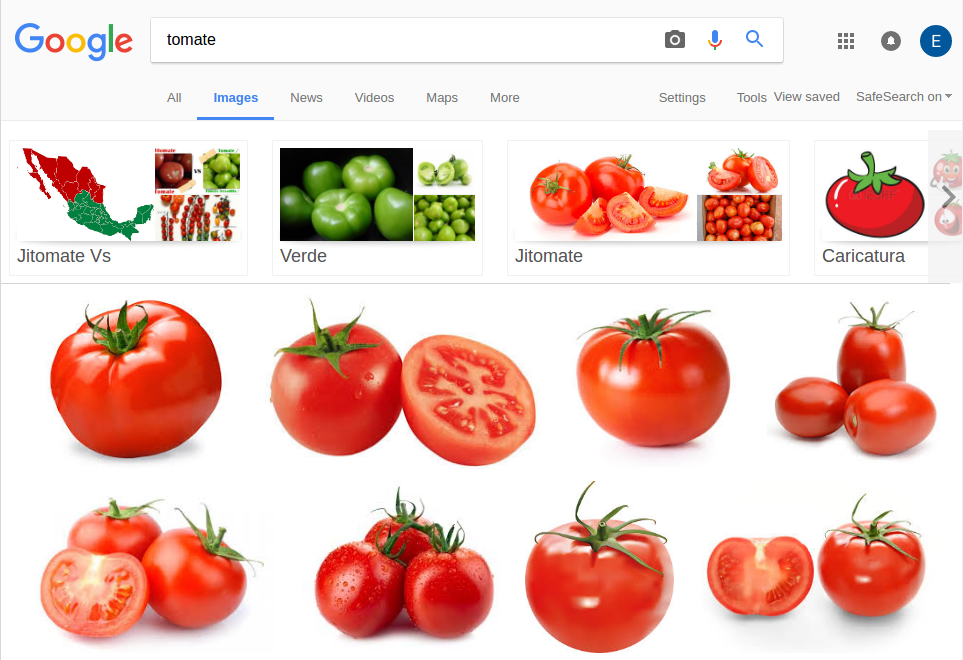
\includegraphics[width=\textwidth]{images/tomate.png}}
    
    \label{resultadoBusca}
  %\end{subfigure}
  
  \legend{\textbf{Fonte:} \citeonline{google0}.}
\end{center}

\end{figure}

A apresentação dos resultados acontece na própria página de resultados. Algumas páginas de resultados do \emph{Google} possuem um componente HTML que exibe grupos relacionados a busca feita. A Figura \ref{resultadoBusca} mostra a região que classifica a busca por tomate em Jitomate Vs, Verde, Jitomate e Caricatura. Esta mesma região será duplicada na página para exibir os resultados do algoritmo. Uma vez que esta região é copiada na página, a aplicação substitui as imagens pelas imagens agrupadas pela aplicação como mostra a Figura \ref{tomateCluster}.

\begin{figure}[htb]
\begin{center}
  %\caption{Imagem colorida ampliada.}
  %\begin{subfigure}[b]{0.6\textwidth}
  \centering
  \caption{Exibição do resultado do algoritmo na própria página.}
      \fbox{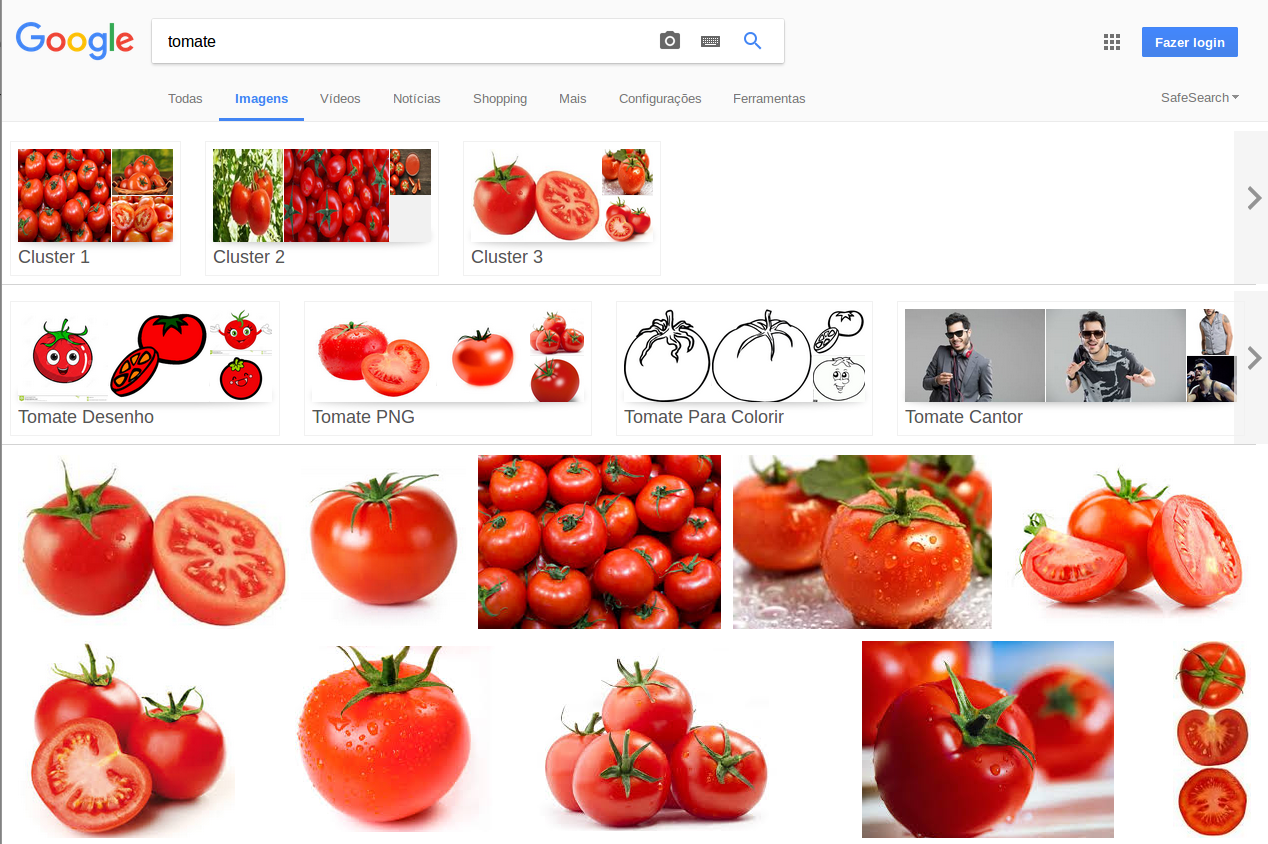
\includegraphics[width=\textwidth]{images/tomateCluster.png}}
    
    \label{tomateCluster}
  %\end{subfigure}
  
  \legend{\textbf{Fonte:} \citeonline{google0}.}
\end{center}

\end{figure}